% !TEX root = ../main.tex

\section{Закон ветра. Изменение ветра с высотой в свободной атм в разных частях циклона и антициклона}
В циклоне $F_{\text{гр}}$ и ветер направлены к центру, в антициклоне - к периферии.
Из-за термического ветра градиентный ветер смещается с высотой так (если предположить, что снизу холод, сверху тепло):
\begin{wrapfigure}[7]{R}{0.51\linewidth}
	\vspace{-8ex}
	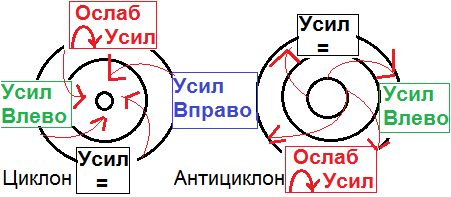
\includegraphics[width=28 mm]{Cyclon}
\end{wrapfigure}

В передней части циклона и на западной периферия антициклона ветер \textcolor{blue}{усиливается и поворачивает в право} \\
В тылу циклона и на восточной периферии антициклона \textcolor{Green}{усиливается и поворачивает влево}\\
В южной части циклона и в северной части антициклона \textbf{усиливается не меняя направление}\\
В северной части циклона и в южной части антициклона \textcolor{red}{ослабевает} На некотором уровне меняет свое направление на противоположное после чего усиливается.

	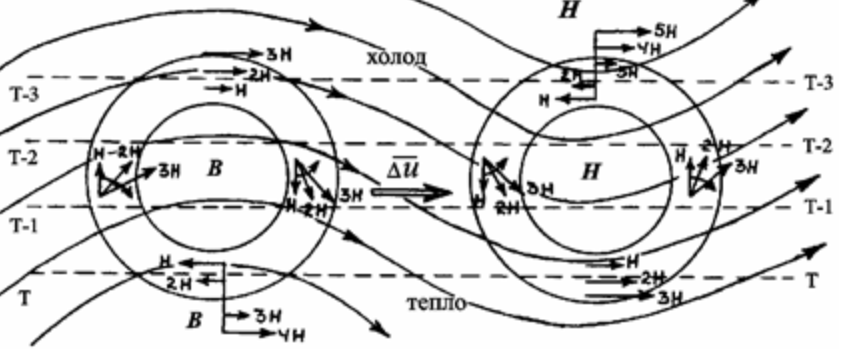
\includegraphics[width=50 mm]{Thermalwind2}

\textbf{Ведущий поток} - ветровой поток однородного напр-ия, который образуется на некоторой высоте (обычно 3-5 км). По нему перемещаются циклоны и антициклоны, приземные центры которых распол-ся под этим потоком. Скорость перемещения бар. систем составляет 80\% от $V_{cp}$ ведущего потока на 3 км или 50\% на 5 км.
\par \textbf{Центр циклона} на высоте смещен относительно произвольного центра в область холода, а \textbf{центр антициклона} - в область тепла.
\par Правое вращение ветра с высотой в свободной атмосфере является признаком наступающего потепления и приближения передней части циклона. Левое вращение характеризует вторжение холодного воздуха и приближение передней части антициклона.